
  \documentclass{beamer}
  \beamertemplatenavigationsymbolsempty
  \setbeamertemplate{footline}[frame number] 
  \setbeamercolor{page number in head/foot}{fg=gray} 
  \usepackage[swedish]{babel}
  \usepackage[utf8]{inputenc}
  \usepackage[T1]{fontenc}
  \usepackage{tgheros, beramono}
  \usepackage{fancyvrb}
  \usepackage{xcolor}
  \definecolor{mygreen}{rgb}{0,0.4,0}
  \definecolor{mylinkcolor}{rgb}{0,0.1,0.5}
  \definecolor{myemphcolor}{rgb}{0,0.4,0.1}
  \definecolor{myalertcolor}{rgb}{0.4,0.1,0}
  \definecolor{eclipsepurple}{rgb}{0.5,0,0.25}
  \definecolor{eclipseblue}{rgb}{0.16,0,1.0}
  \definecolor{eclipsegreen}{rgb}{0,0.5,0}
  \usepackage{listings}

  %%% lingstings specifics:

  \lstdefinelanguage{Scala}{
    morekeywords={abstract,case,catch,class,def,%
      do,else,enum,export,extends,false,final,finally,%
      for,given,if,implicit,import,lazy,match,%
      new,null,object,override,package,%
      private,protected,return,sealed,%
      super,then,throw,trait,true,try,%
      type,val,var,while,with,yield,%
      as, derives, end, extension, infix, inline, opaque, open, transparent, using}, % soft keywords
    otherkeywords={=>,<-,<:,>:,@,=>>,?=>},
    sensitive=true,
    morecomment=[l]{//},
    morecomment=[n]{/*}{*/},
    morestring=[b]",
    morestring=[b]',
    morestring=[b]"""
  }

  \lstset{
      language=Scala,
      tabsize=2,
      basicstyle=\ttfamily,
      keywordstyle=\bfseries\color{eclipsepurple},
      commentstyle=\color{mygreen},
      numberstyle={\footnotesize},
      numbers=none,
      %backgroundcolor=\color{gray!15},
      frame=none, %single,
      rulecolor=\color{black!25},
      %title={\footnotesize\lstname},
      breaklines=false,
      breakatwhitespace=false,
      framextopmargin=2pt,
      framexbottommargin=2pt,
      showstringspaces=false,
      columns=fullflexible,keepspaces
  }

  \lstset{literate=%
  {Å}{{\AA}}1
  {Ä}{{\"A}}1
  {Ö}{{\"O}}1
  {Ü}{{\"U}}1
  {ß}{{\ss}}1
  {ü}{{\"u}}1
  {å}{{\aa}}1
  {ä}{{\"a}}1
  {ö}{{\"o}}1
  {æ}{{\ae}}1
  {ø}{{\o}}1
  {Æ}{{\AE}}1
  {Ø}{{\O}}1
  {`}{{\`{}}}1
  {─}{{\textemdash}}1
  {└}{{|}}1
  {├}{{|}}1
  {│}{{|}}1
  {♠}{{$\spadesuit$}}1
  {♥}{{$\heartsuit$}}1
  {♣}{{$\clubsuit$}}1
  {♦}{{$\diamondsuit$}}1
  }

  \lstnewenvironment{Scala}[1][]{%
      \lstset{#1}%
  }{}  
    
\author{Björn Regnell}
\title{Introduction to Software\\Requirements Engineering}
\usepackage[yyyymmdd]{datetime}
\renewcommand{\dateseparator}{--}
\date{\footnotesize Updated: \today}
\begin{document}
\maketitle

\begin{frame}[fragile]{Who is Björn Regnell?}
\begin{minipage}[t][1.0\textheight]{0.78\textwidth}
\vspace{0pt}
\begin{itemize}
\item Professor in Software Engineering at the Faculty of Engineering, LTH, Lund University, Sweden.
\item Research areas: 
\begin{itemize}
\item Software Engineering
\item Requirements Engineering 
\item Empirical research methods in Software Engineering 
\end{itemize}
\item Current teaching: 
\begin{itemize}
\item Software Requirements Engineering
\item Introduction to Programming in Scala 
\end{itemize}
\item Homepage: 
\begin{itemize}
\item \url{https://cs.lth.se/bjorn-regnell}
\end{itemize}
\end{itemize}
\end{minipage}%
\hspace*{1em}\begin{minipage}[t][1.0\textheight]{0.22\textwidth}
\vspace{0pt}\hfill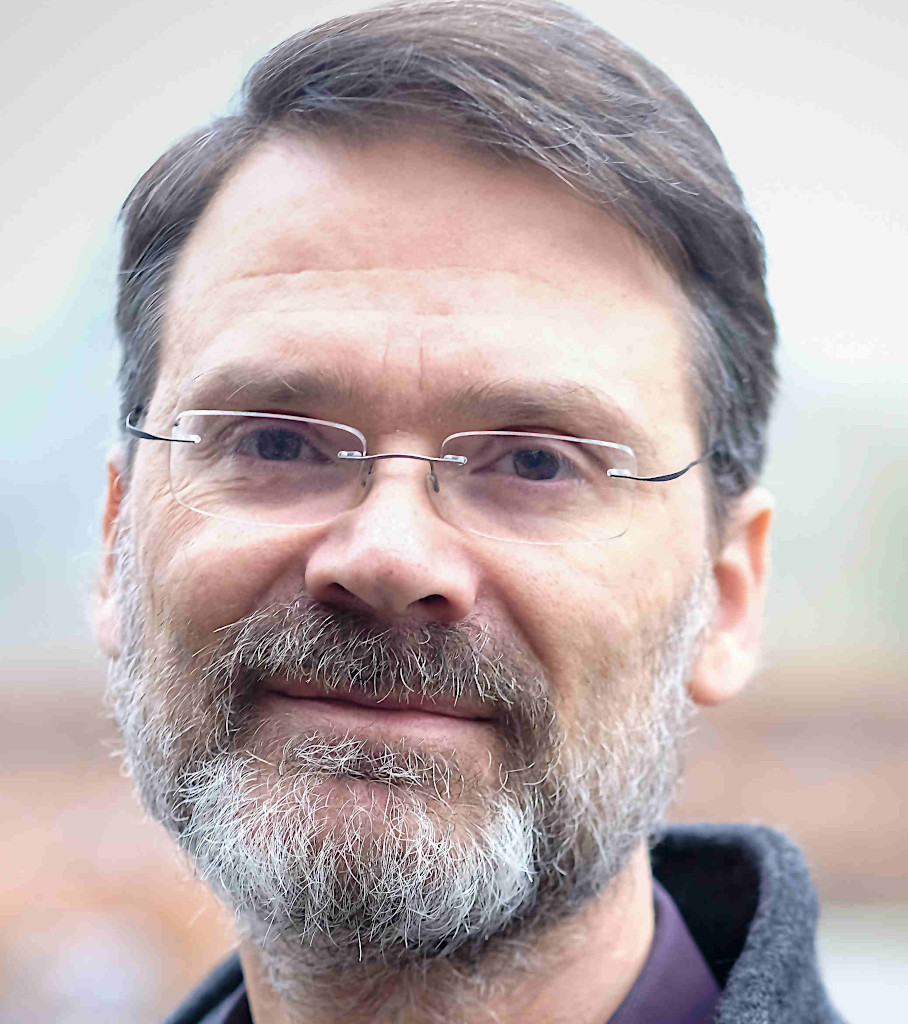
\includegraphics[width=0.9\textwidth]{img/bjorn-regnell}
\end{minipage}%
\end{frame}

\begin{frame}[fragile]{What is Requirements Engineering (RE)?}
\begin{itemize}
\item  Requirements Engineering (RE) is a sub-discipline of Software Engineering (SE) that is focused on the \textit{requirements} of software-intensive systems and their \textit{context}, which includes users and surrounding systems.
\item When you work with anything related to the \textit{decision-making process} of software development and its \emph{underlying intentions} you are doing requirements engineering.
\end{itemize}
\end{frame}

\begin{frame}[fragile]{What is a requirement?}
\begin{itemize}
\item Something needed or wanted.
\item A documented representation of \\something needed or wanted.
\item The word ''requirement'' can have different meanings:
\begin{itemize}
\item ... must, wish, idea, design detail, rationale, ...
\item The most general meaning of ''requirement'':
\item[] \emph{any} kind of information entity used in RE
\end{itemize}
\end{itemize}
\end{frame}

\begin{frame}[fragile]{Activities in Requirements Engineering}
\begin{itemize}
\item \textbf{Elicitation}: learn, invent and agree.
\item \textbf{Specification}: represent, communicate \& make persistent.
\item \textbf{Validation}: check if requirements are good.
\item \textbf{Selection}: prioritize, decide and plan.
\end{itemize}
\vspace*{1em}
Often conducted concurrently and iteratively.
\end{frame}

\begin{frame}[fragile]{Aspects of Requirements Modelling}
\begin{itemize}
\item Qualities of requirements models
\item Requirements on functionality and quality
\item Requirements at Different Levels
\end{itemize}
\end{frame}

\begin{frame}[fragile]{Quality of Requirements Models}
What is a good requirements model? good enough
\\ \vspace*{1em}Examples of quality aspects fulfilled to some degree:
\begin{itemize}
\item \textbf{Correctness}: reflect the expected, intended behavior
\item \textbf{Unambiguity}: stakholders have similar interpretation
\item \textbf{Completeness}: most important, relevant aspects included
\item \textbf{Consistency}: no contradictions among requirements
\item \textbf{Conciseness}: suitable level of abstraction and detail 
\item \textbf{Comprehensibility}: understood by stakeholders 
\item \textbf{Verifiability}: possible to check fulfillment 
\item \textbf{Feasibility}: possible to implement, value to justifiable cost 
\item \textbf{Traceability}: can be referred to, can find its origin
\item \textbf{Modifyability}: easy to change, good structure
\item \textbf{Ranked}: includes evaluations of importance and stability
\end{itemize}
\end{frame}

\begin{frame}[fragile]{xx}
\begin{itemize}
\item xx 
\begin{itemize}
\item xx 
\end{itemize}
\end{itemize}
\end{frame}

\begin{frame}[fragile]{xx}
\begin{itemize}
\item xx 
\begin{itemize}
\item xx 
\end{itemize}
\end{itemize}
\end{frame}

\begin{frame}[fragile]{xx}
\begin{itemize}
\item xx 
\begin{itemize}
\item xx 
\end{itemize}
\end{itemize}
\end{frame}

\begin{frame}[fragile]{xx}
\begin{itemize}
\item xx 
\begin{itemize}
\item xx 
\end{itemize}
\end{itemize}
\end{frame}

\begin{frame}[fragile]{xx}
\begin{itemize}
\item xx 
\begin{itemize}
\item xx 
\end{itemize}
\end{itemize}
\end{frame}

\begin{frame}[fragile]{xx}
\begin{itemize}
\item xx 
\begin{itemize}
\item xx 
\end{itemize}
\end{itemize}
\end{frame}

\begin{frame}[fragile]{xx}
\begin{itemize}
\item xx 
\begin{itemize}
\item xx 
\end{itemize}
\end{itemize}
\end{frame}



    
\end{document}

